\documentclass[tikz, border=10pt, multi=tikzpicture]{standalone}
\usepackage[utf8]{inputenc}
\usetikzlibrary{shapes.geometric, arrows.meta, positioning, calc, shadows}

% Define colors
\definecolor{primary}{RGB}{0, 102, 204}
\definecolor{secondary}{RGB}{0, 153, 76}
\definecolor{accent}{RGB}{204, 0, 0}
\definecolor{background}{RGB}{240, 247, 255}
\definecolor{modulebox}{RGB}{230, 230, 230}

% Define TikZ styles
\tikzset{
    base/.style={draw, thick, align=center, font=\small\sffamily, fill=white, drop shadow},
    process/.style={base, rectangle, minimum width=3.5cm, minimum height=1cm, fill=blue!10},
    module/.style={base, rectangle, rounded corners, minimum width=4cm, minimum height=1.5cm, fill=green!10, dashed},
    decision/.style={base, diamond, aspect=2, minimum width=3.5cm, fill=orange!10},
    io/.style={base, trapezium, trapezium left angle=70, trapezium right angle=110, minimum width=3.5cm, minimum height=1cm, fill=gray!10},
    cloud/.style={base, ellipse, minimum width=2.5cm, minimum height=0.8cm, fill=yellow!10},
    arrow/.style={-Stealth, thick, draw=black!70}
}

\begin{document}

% ---------------- Overall Architecture ----------------
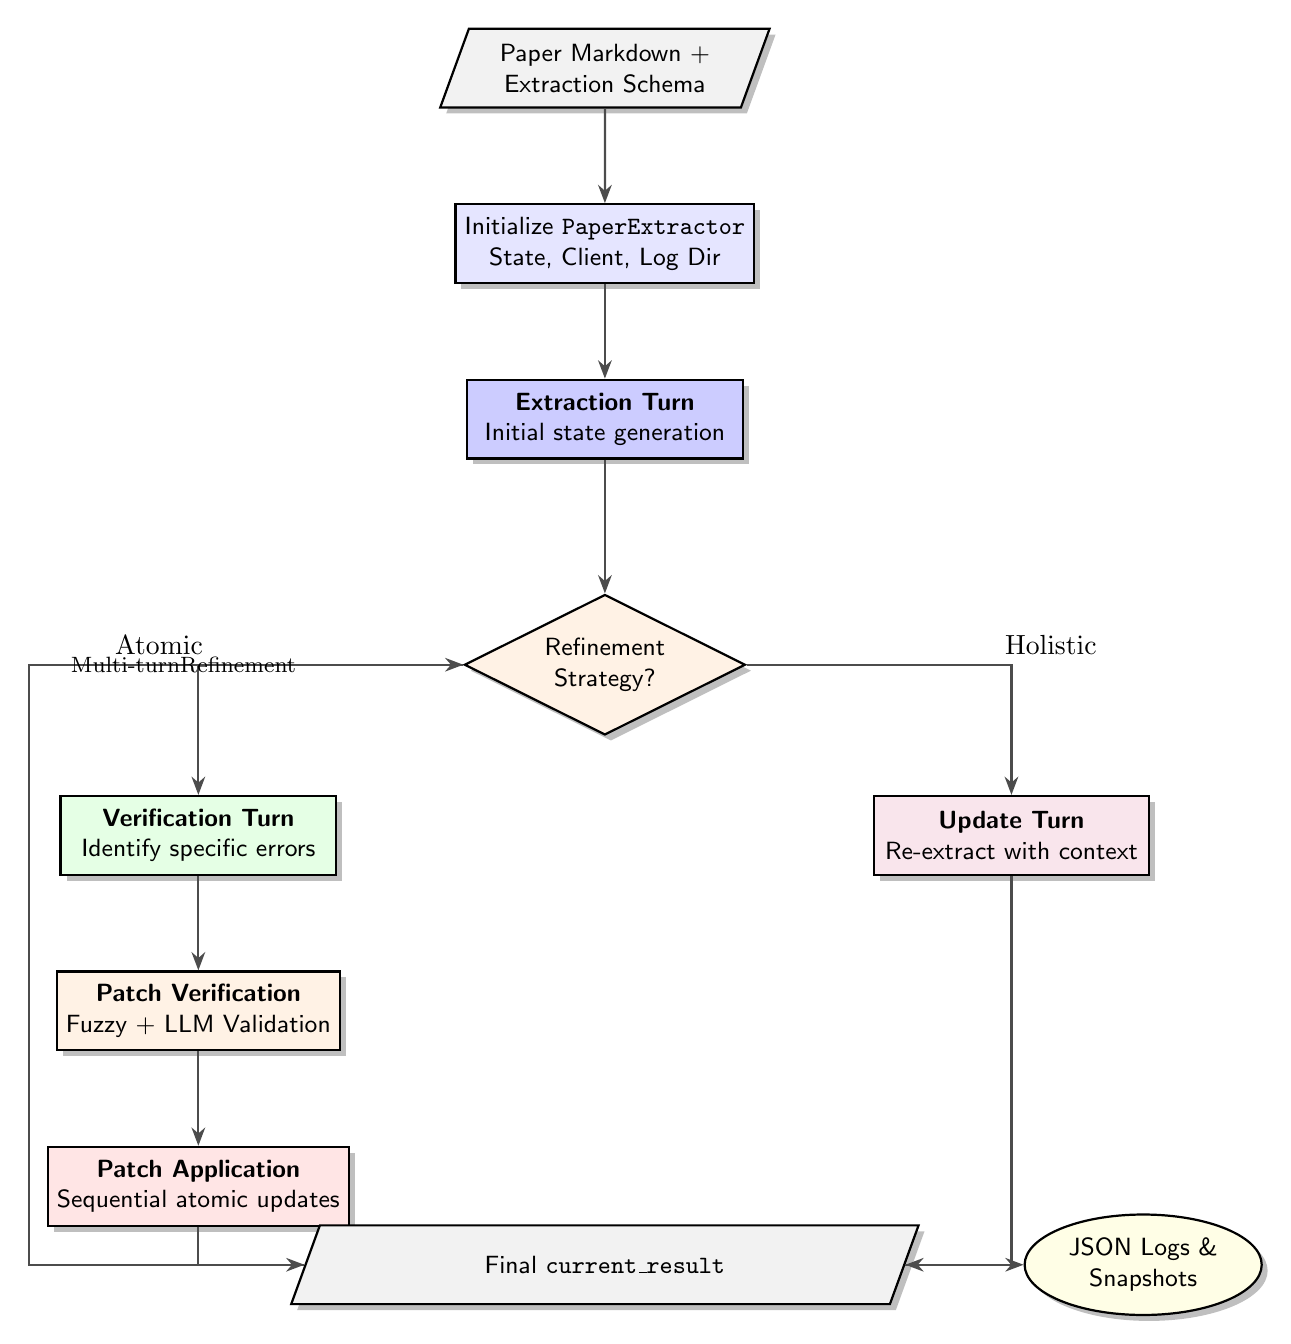
\begin{tikzpicture}[node distance=1.2cm and 1.5cm]
    % Nodes
    \node (input) [io] {Paper Markdown + \\ Extraction Schema};
    \node (init) [process, below=of input] {Initialize \texttt{PaperExtractor} \\ State, Client, Log Dir};
    
    % Extraction Phase
    \node (extraction) [process, below=of init, fill=blue!20] {\textbf{Extraction Turn} \\ Initial state generation};
    
    % Branching refinement
    \node (refine_dec) [decision, below=of extraction, yshift=-0.5cm] {Refinement \\ Strategy?};

    % Path A: Atomic (Verification)
    \node (verification) [process, below left=of refine_dec, xshift=-1cm, fill=green!10] {\textbf{Verification Turn} \\ Identify specific errors};
    \node (patch_verify) [process, below=of verification, fill=orange!10] {\textbf{Patch Verification} \\ Fuzzy + LLM Validation};
    \node (application) [process, below=of patch_verify, fill=red!10] {\textbf{Patch Application} \\ Sequential atomic updates};

    % Path B: Holistic (Update)
    \node (update) [process, below right=of refine_dec, xshift=1cm, fill=purple!10] {\textbf{Update Turn} \\ Re-extract with context};
    
    \node (output) [io, below=of refine_dec, yshift=-5cm] {Final \texttt{current\_result}};
    
    \node (logs) [cloud, right=of output] {JSON Logs \& \\ Snapshots};

    % Flows
    \draw [arrow] (input) -- (init);
    \draw [arrow] (init) -- (extraction);
    \draw [arrow] (extraction) -- (refine_dec);
    
    % Path A flows
    \draw [arrow] (refine_dec) -| node[anchor=south, xshift=-0.5cm] {Atomic} (verification);
    \draw [arrow] (verification) -- (patch_verify);
    \draw [arrow] (patch_verify) -- (application);
    \draw [arrow] (application) |- (output);
    
    % Path B flows
    \draw [arrow] (refine_dec) -| node[anchor=south, xshift=0.5cm] {Holistic} (update);
    \draw [arrow] (update) |- (output);
    
    \draw [arrow] (output.east) -- (logs.west);
    
    % Loop back for multi-turn
    \draw [arrow] (output.west) -- ++(-3.5,0) |- (refine_dec.west);
    \node [left=of refine_dec, xshift=-0.5cm, font=\footnotesize] {Multi-turn \\ Refinement};
\end{tikzpicture}

% ---------------- Extraction Module Structure ----------------
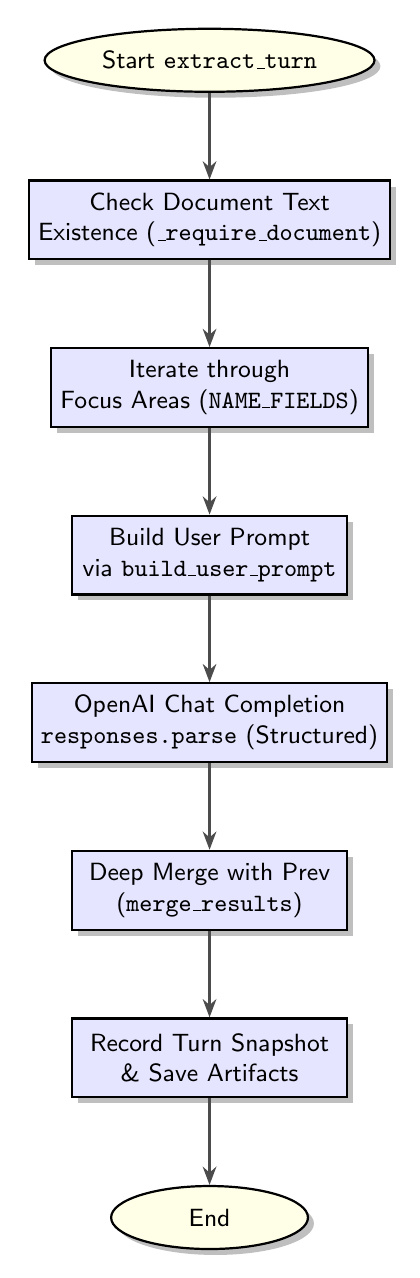
\begin{tikzpicture}[node distance=1.1cm]
    \node (start) [cloud] {Start \texttt{extract\_turn}};
    \node (check) [process, below=of start] {Check Document Text \\ Existence (\texttt{\_require\_document})};
    \node (loop) [process, below=of check] {Iterate through \\ Focus Areas (\texttt{NAME\_FIELDS})};
    \node (prompt) [process, below=of loop] {Build User Prompt \\ via \texttt{build\_user\_prompt}};
    \node (api) [process, below=of prompt] {OpenAI Chat Completion \\ \texttt{responses.parse} (Structured)};
    \node (merge) [process, below=of api] {Deep Merge with Prev \\ (\texttt{merge\_results})};
    \node (snapshot) [process, below=of merge] {Record Turn Snapshot \\ \& Save Artifacts};
    \node (end) [cloud, below=of snapshot] {End};

    \draw [arrow] (start) -- (check);
    \draw [arrow] (check) -- (loop);
    \draw [arrow] (loop) -- (prompt);
    \draw [arrow] (prompt) -- (api);
    \draw [arrow] (api) -- (merge);
    \draw [arrow] (merge) -- (snapshot);
    \draw [arrow] (snapshot) -- (end);
\end{tikzpicture}

% ---------------- Update Module Structure ----------------
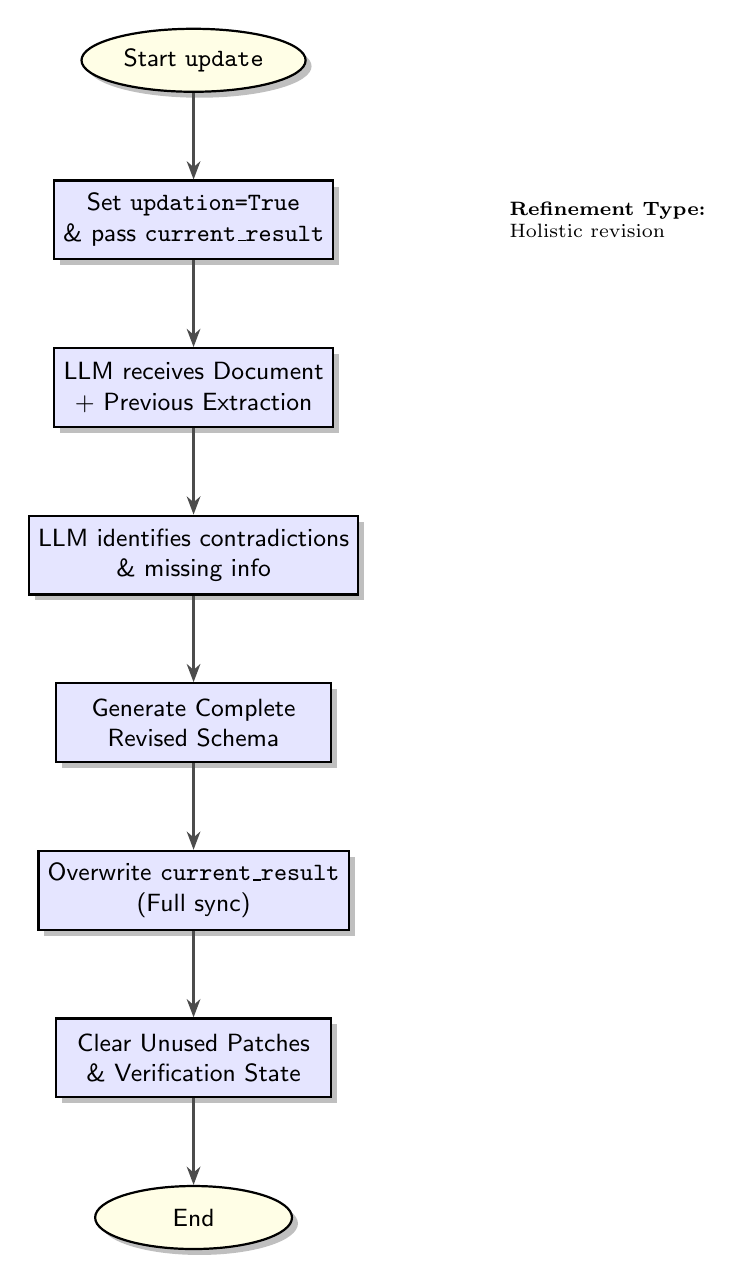
\begin{tikzpicture}[node distance=1.1cm]
    \node (start) [cloud] {Start \texttt{update}};
    \node (prep) [process, below=of start] {Set \texttt{updation=True} \\ \& pass \texttt{current\_result}};
    \node (prompt) [process, below=of prep] {LLM receives Document \\ + Previous Extraction};
    \node (logic) [process, below=of prompt] {LLM identifies contradictions \\ \& missing info};
    \node (gen) [process, below=of logic] {Generate Complete \\ Revised Schema};
    \node (apply) [process, below=of gen] {Overwrite \texttt{current\_result} \\ (Full sync)};
    \node (clear) [process, below=of apply] {Clear Unused Patches \\ \& Verification State};
    \node (end) [cloud, below=of clear] {End};

    \draw [arrow] (start) -- (prep);
    \draw [arrow] (prep) -- (prompt);
    \draw [arrow] (prompt) -- (logic);
    \draw [arrow] (logic) -- (gen);
    \draw [arrow] (gen) -- (apply);
    \draw [arrow] (apply) -- (clear);
    \draw [arrow] (clear) -- (end);
    
    \node [right=of prep, xshift=1cm, font=\scriptsize, align=left] {\textbf{Refinement Type:} \\ Holistic revision};
\end{tikzpicture}

% ---------------- Verification Module Structure ----------------
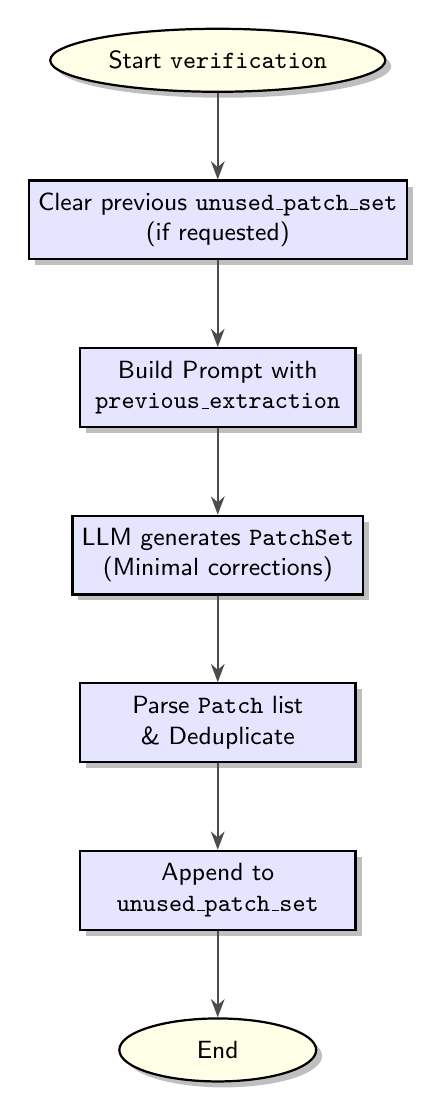
\begin{tikzpicture}[node distance=1.1cm]
    \node (start) [cloud] {Start \texttt{verification}};
    \node (clear) [process, below=of start] {Clear previous \texttt{unused\_patch\_set} \\ (if requested)};
    \node (prompt) [process, below=of clear] {Build Prompt with \\ \texttt{previous\_extraction}};
    \node (api) [process, below=of prompt] {LLM generates \texttt{PatchSet} \\ (Minimal corrections)};
    \node (parse) [process, below=of api] {Parse \texttt{Patch} list \\ \& Deduplicate};
    \node (state) [process, below=of parse] {Append to \\ \texttt{unused\_patch\_set}};
    \node (end) [cloud, below=of state] {End};

    \draw [arrow] (start) -- (clear);
    \draw [arrow] (clear) -- (prompt);
    \draw [arrow] (prompt) -- (api);
    \draw [arrow] (api) -- (parse);
    \draw [arrow] (parse) -- (state);
    \draw [arrow] (state) -- (end);
\end{tikzpicture}

% ---------------- Patch Verification Structure ----------------
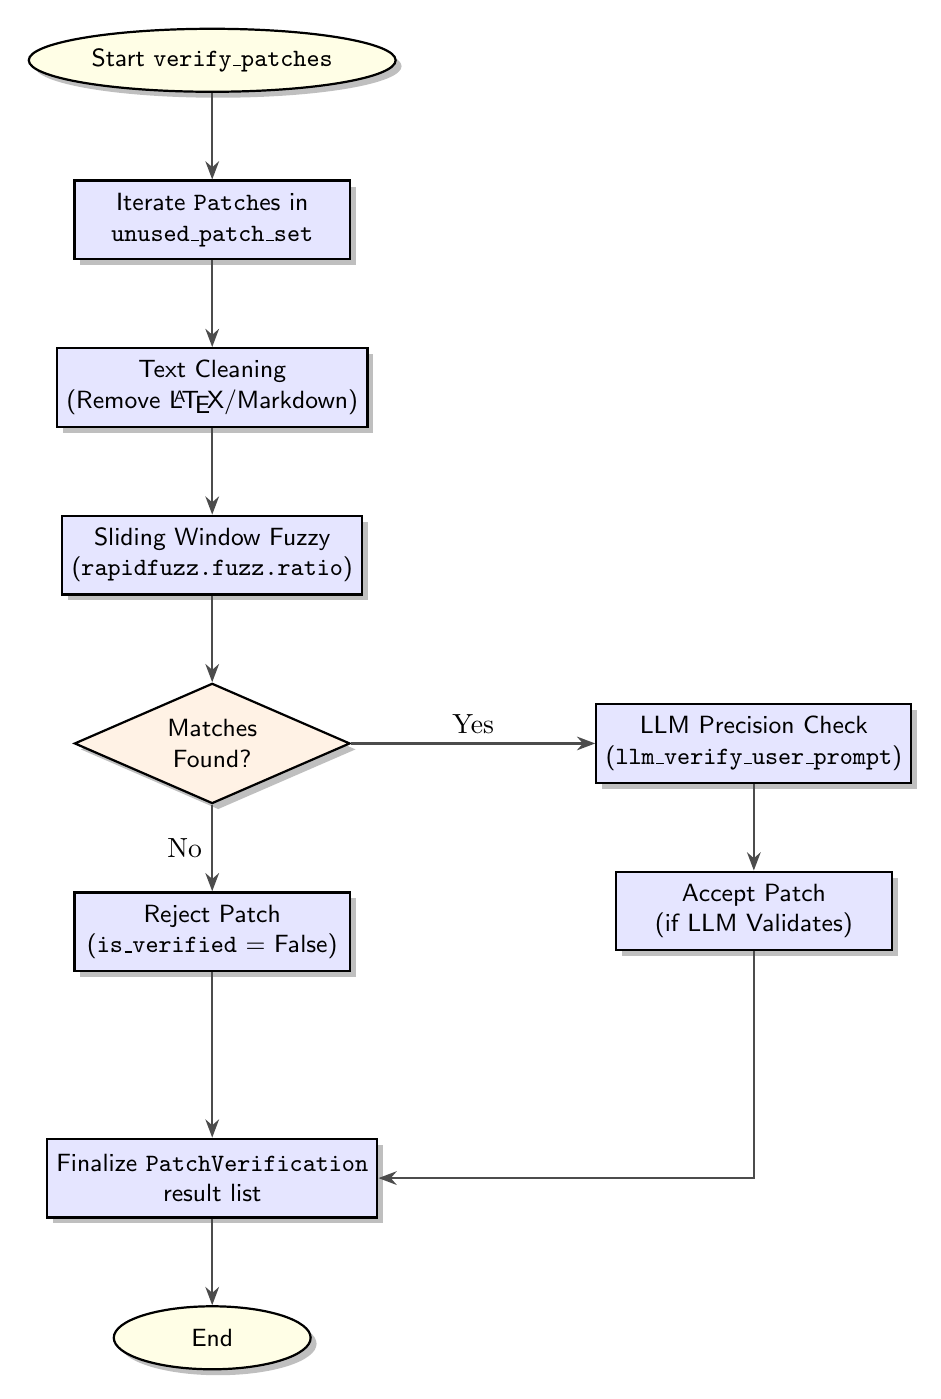
\begin{tikzpicture}[node distance=1.1cm]
    \node (start) [cloud] {Start \texttt{verify\_patches}};
    \node (loop) [process, below=of start] {Iterate \texttt{Patch}es in \\ \texttt{unused\_patch\_set}};
    
    \node (clean) [process, below=of loop] {Text Cleaning \\ (Remove \LaTeX/Markdown)};
    \node (fuzzy) [process, below=of clean] {Sliding Window Fuzzy \\ (\texttt{rapidfuzz.fuzz.ratio})};
    \node (matches) [decision, below=of fuzzy] {Matches \\ Found?};
    
    \node (llm_verify) [process, right=of matches, xshift=2cm] {LLM Precision Check \\ (\texttt{llm\_verify\_user\_prompt})};
    \node (failed) [process, below=of matches] {Reject Patch \\ (\texttt{is\_verified} = False)};
    
    \node (success) [process, below=of llm_verify] {Accept Patch \\ (if LLM Validates)};
    
    \node (collect) [process, below=of failed, yshift=-1cm] {Finalize \texttt{PatchVerification} \\ result list};
    \node (end) [cloud, below=of collect] {End};

    \draw [arrow] (start) -- (loop);
    \draw [arrow] (loop) -- (clean);
    \draw [arrow] (clean) -- (fuzzy);
    \draw [arrow] (fuzzy) -- (matches);
    \draw [arrow] (matches) -- node[anchor=south] {Yes} (llm_verify);
    \draw [arrow] (matches) -- node[anchor=east] {No} (failed);
    \draw [arrow] (llm_verify) -- (success);
    \draw [arrow] (failed) -- (collect);
    \draw [arrow] (success) |- (collect);
    \draw [arrow] (collect) -- (end);
\end{tikzpicture}

% ---------------- Patch Application Structure ----------------
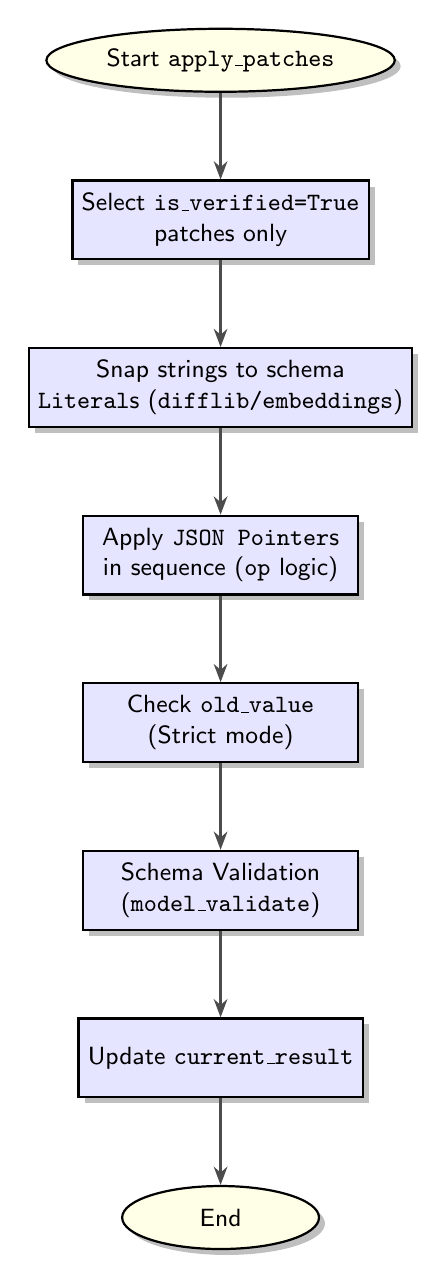
\begin{tikzpicture}[node distance=1.1cm]
    \node (start) [cloud] {Start \texttt{apply\_patches}};
    \node (filter) [process, below=of start] {Select \texttt{is\_verified=True} \\ patches only};
    \node (normalize) [process, below=of filter] {Snap strings to schema \\ \texttt{Literal}s (\texttt{difflib/embeddings})};
    \node (sequential) [process, below=of normalize] {Apply \texttt{JSON Pointer}s \\ in sequence (\texttt{op} logic)};
    \node (mismatch) [process, below=of sequential] {Check \texttt{old\_value} \\ (Strict mode)};
    \node (validate) [process, below=of mismatch] {Schema Validation \\ (\texttt{model\_validate})};
    \node (update) [process, below=of validate] {Update \texttt{current\_result}};
    \node (end) [cloud, below=of update] {End};

    \draw [arrow] (start) -- (filter);
    \draw [arrow] (filter) -- (normalize);
    \draw [arrow] (normalize) -- (sequential);
    \draw [arrow] (sequential) -- (mismatch);
    \draw [arrow] (mismatch) -- (validate);
    \draw [arrow] (validate) -- (update);
    \draw [arrow] (update) -- (end);
\end{tikzpicture}

\end{document}

